\chapter{Git}\label{cha:git}
In diesem Kapitel werden die wesentlichsten Grundlagen und Befehle
beschrieben, um mit Git Dateien zu verwalten. Zunächst wird mit einfachen
Befehlen ein Git-Repository erstellt und später am Beispiel dieses Repositories
auf weitere Eigenschaften und Befehle eingegangen.

\section{Grundlagen}\label{gitbasics}
Hier wird beispielhaft ein Repository \textit{git-example} mit einem
Skript (\texttt{git-stats}) erstellt, welches ein paar einfache Statistiken
über die Autoren eines Git-Repositories erzeugt.

Alle Beispiele werden auf der Linux Kommandozeile durchgeführt. Git ist für
alle gängigen Linux Derivate verfügbar. Die Autoren von \cite[S.~12-14]{progit}
gehen auf weitere Details zur Installation von Git auf anderen Betriebssystemen
ein.

Die in den Beispielen eingesetzte Version von Git ist 2.15.0.

\eqlst{listings/git_version.lst}{lst:gitversion}{Die Version von Git ausgeben}

Der folgende Abschnitt basiert zum Teil auf den Ausführungen der Autoren aus
\cite[S.22-57]{gitosp}.

\subsection{Konfiguration}\label{gitconfig}
Zu Beginn werden einige grundlegende Konfigurationen vorgenommen. So werden,
damit die Nachvollziehbarkeit gewährleistet ist, zunächst Name und Mailadresse
des Benutzers konfiguriert. Auch ist die farbliche Darstellung der Ausgaben
durchaus hilfreich. Hier kann Git so konfiguriert werden, dass die Farbausgabe
automatisch unterdrückt wird, sollte die Ausgabe in eine Datei umgeleitet
werden.

\eqlst{listings/git_init_config.lst}{lst:gitinitconfig}{Die erste Git Konfiguration}

Die \textit{global} eingestellten Optionen können ebenfalls direkt in der Datei
\texttt{\textasciitilde/.gitconfig} eingesehen und bearbeitet werden.
Zusätzlich können für jedes Repository spezifische Konfigurationen vorgenommen
werden. Hierzu muss der Parameter \texttt{\-\-global} entfernt werden. Die
zugehörige Konfigurationsdatei findet sich in jedem Repository unter dem Pfad
\texttt{.git/config}.

\subsection{Erstellen eines Repositories}\label{startup}
Damit Dateien nun mit Git versioniert werden können, muss ein (lokales)
\gls{repository} erstellt werden:

\eqlst{listings/git_init.lst}{lst:gitinit}{Ein lokales Repository anlegen}

Existiert das Verzeichnis \texttt{git-example.git} noch nicht, wird es durch
den Befehl angelegt. Zusätzlich wird innerhalb von \texttt{git-example.git}
noch ein weiteres Verzeichnis \texttt{.git} erzeugt, in dem neben der
Konfiguration alle Daten abgelegt werden, die Git zur weiteren Verwaltung des
\glspl{repository} benötigt.

Um den Status des aktuell erzeugten \glspl{repository} auszugeben, kann der
Befehl \texttt{\$ git status} verwendet werden:

\eqlst{listings/git_status.lst}{lst:gitstatus}{Den Status eines Repositories ausgeben}

Die von Git erzeugte Ausgabe macht darauf aufmerksam, dass noch keine Commits
erzeugt wurden und dass man nun neue Dateien erstellen und hinzufügen kann.

\subsection{Die ersten Commits}\label{sec:first_commits}

Hier werden nun die ersten Dateien zu dem Repository hinzugefügt. Dazu werden
mit folgendem Befehl, zwei Dateien aus dem Internet heruntergeladen. Zuvor wird
mit dem Befehl \texttt{\$ mkdir helpers} ein Unterordner in dem erzeugten
Repository angelegt.

\eqlst{listings/downloads.lst}{lst:downloads}{Herunterladen der Beispieldateien}

Ab jetzt können die Dateien mit Git verwaltet werden. Ein erstes Hinzufügen
einer Datei mit dem Befehl \texttt{\$ git add LICENSE} führt zu folgender
Ausgabe von \texttt{\$ git status}:

\eqlst{listings/add_first_file.lst}{lst:add_first_file}{Eine erste Datei hinzufügen}

Die Ausgabe macht darauf aufmerksam, dass zum Einen eine neue Datei zum Commit
vorgemerkt ist und dass sich zum Anderen noch eine Datei im Verzeichnis
befindet, die noch nicht mit Git verwaltet wird. Hierbei ist anzumerken, dass
Git auch die vorgemerkte Datei noch nicht versioniert. Dazu muss zuerst ein
Commit erstellt werden. Darauf wie Git hier unterscheidet, wird später
(Abschnitt \ref{sec:trees}) eingegangen.

Der erste Commit in dem angelegten Repository wird mit dem Befehl \texttt{\$
git commit} erzeugt. Eine Bemerkung zu dem Commit kann, je nach
voreingestelltem Systemeditor jetzt eingegeben oder optional mit dem Parameter
\texttt{-m} direkt auf der Kommandozeile (Listing \ref{lst:git_first_commit})
übergeben werden. In der Bemerkung wird die erste Zeile als Betreff und
getrennt durch eine Leerzeile, alle weiteren Zeilen als ausführliche
Beschreibung verwendet. Dieses Format ist in den meisten
Versionskontrollsystemen üblich.

\eqlst{listings/git_first_commit.lst}{lst:git_first_commit}{Ein erster Commit}

Darüber hinaus bietet es sich an, beim Erstellen solcher Bemerkungen gewisse
Regeln einzuhalten. Beispielsweise beschreiben Jez Humble und David Farley in
\cite[S.~37]{cd} eine Situation, in der es sinnvoll ist, nicht nur zu wissen,
was der Autor geändert hat, sondern auch warum und in welchem Kontext. Wenn
nicht klar ist, was der Autor sich bei Änderungen gedacht hat oder
Zusammenhänge nicht aus dem Commit hervorgehen, kann ein gefundener und
behobener Fehler vor dem Veröffentlichen einer Softwareversion durchaus zu
Folgefehlern führen. Solche Situationen enden nicht selten darin, dass viele
Stunden Arbeit investiert werden müssen, um diese zu bereinigen.
\cite[S.~37]{cd}

Nachdem der erste Commit erzeugt wurde, kann dieser nun mit \texttt{\$ git
show} (Abschnitt \ref{sec:arch}) betrachtet werden. In diesem Fall wurde
beispielhaft eine etwas ausführlichere Bemerkung für den Commit gewählt:

\eqlst{listings/git_show_first_commit.lst}{lst:git_show_first_commit}{Anzeige
des ersten Commits}

Mit \texttt{\$ git show} können alle wichtigen Informationen eines Commits
eingesehen werden. Neben Zeitpunkt, Autor und Beschreibung beinhaltet dieser
auch die \textit{Commit-ID} (Abschnitt \ref{sec:commit}). Die weiteren
Informationen werden in einem Format namens
\textit{Unified-Diff}\footnote{Details zu dem \textit{Unified-Diff} Format
stellen die Autoren von \textit{GNU diffutils} unter
\cite[S.~12-13]{paper:diffutils} zur Verfügung.} dargestellt. \cite[25]{gitosp}

Mit \texttt{\$ git add} wird nun eine zweite Datei hinzugefügt:

\eqlst{listings/git_add_second_file.lst}{lst:git_add_second_file}{Eine weitere
Datei hinzufügen}

Anschließend wird ein weiterer \gls{commit} erzeugt:

\eqlst{listings/commit_git-stats.lst}{lst:commit_git-stats}{Hinzufügen einer
weiteren Datei}

Mit den beiden zuvor ausgeführten Commits, wurde eine, wenn auch
kurze, Historie erstellt. Um diese zu untersuchen, dienen die Befehle
\texttt{\$ git whatchanged}\footnote{Der Befehl \texttt{\$ git whatchanged}
stammt aus frühen Zeiten von Git und ist eigentlich der heutige Befehl
\texttt{\$ git log} mit einigen Parametern, um die Ausgabe entsprechend zu
formatieren.} oder \texttt{\$ git log}. Hierauf wird in Abschnitt \ref{sec:arch}
weiter eingegangen. Für diesen Fall aber ist \texttt{\$ git whatchanged}
ausreichend:

\eqlst{listings/first_git_whatchanged.lst}{lst:first_git_whatchanged}{Untersuchen
der Historie mit \texttt{whatchanged}}

Die Ausgabe wird im sogenannten \textit{raw} Format dargestellt. Es werden alle
Commits mit Informationen über den Autor, Commit-ID, Zeit und den veränderten
Dateien in zeitlicher Reihenfolge dargestellt. Die konkreten Veränderungen am
Inhalt der Dateien werden hier nicht dargestellt.

Erwähnenswert ist noch, dass Git im Gegensatz zu anderen
Versionskontrollsystemen die Dateiberechtigungen speichert. Die Ausgabe des
letzten Commits (Listing \ref{lst:commit_git-stats}) enthält folgende Zeile:

\eqlst{listings/create_mode.lst}{lst:create_mode}{Berechtigungen einer Datei}

Diese Ausgabe beschreibt, dass es sich hierbei um eine normale Datei handelt (100),
die mit einer unter Unix üblichen Berechtigung (664) angelegt ist. Damit
diese Datei aber entsprechend ausführbar ist, muss noch ein weiterer
Commit, mit einer Änderung an den Dateiberechtigungen, erzeugt werden:

\eqlst{listings/git_commit_all.lst}{lst:git_commit_all}{Einen Commit mit allen
Änderungen anzeigen}

Mit dem zuvor ausgeführten Befehl wurde ein Commit erzeugt, ohne die
Änderungen vorher mit \texttt{\$ git add} hinzuzufügen. Der Parameter
\texttt{-a} bewirkt hier, dass alle vorhandenen Änderungen zu einem Commit
zusammengefasst werden und nicht einzeln hinzugefügt werden müssen. Zu beachten
ist allerdings, dass Dateien, die Git noch nicht kennt, davon nicht betroffen
sind. Diese müssen nach wie vor zuerst mit \texttt{\$ git add} hinzugefügt
werden.

Abschließend erhält der letzte Commit noch eine Markierung bzw. einen \gls{tag}.

\eqlst{listings/git_first_tag.lst}{lst:git_first_tag}{Anlegen eines Tags}

Damit wurde ein \gls{tag} mit dem Namen \texttt{tags/0.0.1} angelegt,
der den letzten Commit bzw. \textit{\gls{HEAD}} referenziert:

\eqlst{listings/git_list_first_tag.lst}{lst:git_list_first_tag}{Auflisten von
lokalen Tags}

Auf den weiteren Umgang mit Tags und die unterschiedlichen Arten von Tags, wird
in den Abschnitten \ref{sec:managetags} und \ref{sec:tagobject} eingegangen.

\subsection{Verteiltes Git}\label{sec:distributed}
In diesem Abschnitt wird das Arbeiten mit entfernten \glspl{repository}
gezeigt (Abbildung \ref{fig:centralworkflow}). Die wesentliche Funktionsweise
von Git ist auf kollaborative Arbeit an \glspl{repository} ausgelegt (Abschnitt
\ref{sec:kernel}).

\begin{figure}[h]
  \centering
  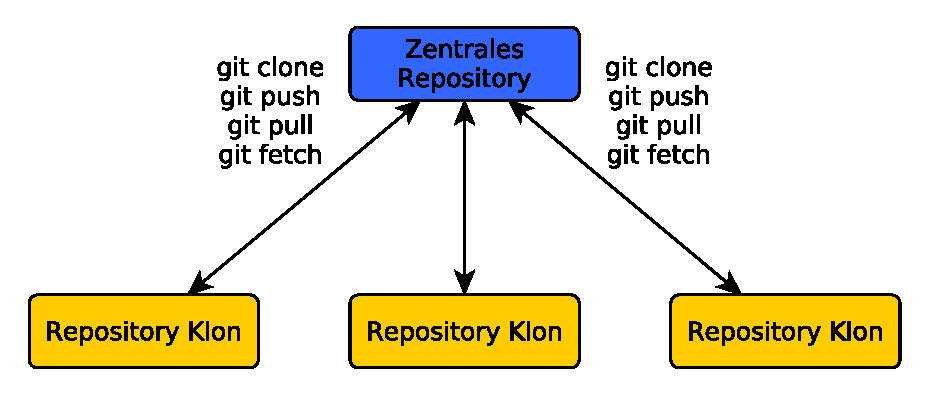
\includegraphics[scale=0.70]{images/workflow.eps}
  \caption{Zentraler Workflow. Angelehnt an \cite[S.~138]{gitosp}}.
  \label{fig:centralworkflow}
\end{figure}

\subsubsection{Erstellen eines Klons}\label{sec:gitclone}
Um eine lokale Kopie eines entfernten Repositories zu erstellen bzw. ein
Repository zu klonen, benötigt man den Befehl \texttt{\$ git clone}. Zum
Transport über das Netzwerk können verschiedene Protokolle benutzt werden.
Unterstützt werden \textit{ssh, git, http[s], ftp[s]} und \textit{file}. Eine
entsprechende \gls{repourl} kann neben dem Protokoll noch den Pfad des
Repositories, einen Benutzernamen oder einen Port enthalten:

\eqlst{listings/git_url.lst}{lst:git_url}{Git Repository Url syntax}

Besonderheiten gibt es für das Klonen lokaler Repositories und solcher, die über
über \gls{sshell}(\acrshort{ssh}) geklont werden. Hier gibt es jeweils eine
Kurzform. Für das Klonen über \acrshort{ssh} muss das Protokoll nicht mit
angegeben werden und bei lokal erreichbaren Repositories kann vollständig auf
die Angabe einer Adresse verzichtet werden. Hier reicht einfach die Angabe
eines Pfads \texttt{/pfad/zum/repo}.

Das Beispiel aus Abschnitt \ref{sec:first_commits} ist als
Repository verfügbar und kann mit folgendem Befehl geklont werden.

\eqlst{listings/git_clone.lst}{lst:git_clone}{Ein Repository klonen}

Git speichert die Herkunft des entfernten \glspl{repository} ebenfalls in der
Datei \texttt{.git/config}:

\eqlst{listings/remote_reference.lst}{lst:remote_reference}{Konfiguration eines
entfernten Repositories anzeigen}

Die gleichen Informationen werden mit Hilfe des Git Befehls \texttt{\$ git
remote} ausgegeben:

\eqlst{listings/git_remote.lst}{lst:git_remote}{Informationen eines entfernten
Repositories anzeigen}

In Listing \ref{lst:git_remote} wird zum Einen der Name, in diesem Fall
\textit{origin}, ausgegeben und zum Anderen, aufgrund der Verwendung des
Parameters \texttt{-v}, auch der Pfad zum entfernten Repository. Mit \texttt{\$
git remote} können weitere entfernte Repositories unter anderem Namen
konfiguriert werden\footnote{Hierzu siehe \texttt{\$ git help remote}}. Ebenso
wird standardmäßig der \gls{branch} \textit{master} konfiguriert und als
sogenannter \textit{remote-tracking-branch} eingerichtet. Diese Branches verfolgen
die Änderungen gleichnamiger Branches aus den entfernten \glspl{repository}
und werden bei einer Synchronisation automatisch durch Git
aktualisiert. \cite[S.~141-143]{gitosp}

Das weitere Bearbeiten des Repositoryinhalts kann wie in Abschnitt
\ref{sec:first_commits} beschrieben durchgeführt werden.

\subsubsection{Änderungen übertragen}\label{sec:pushchanges}
Um Daten in ein entferntes Repository zu übertragen, wird der Befehl \texttt{\$
git push} benutzt. Als Standardziel wird das Repository verwendet, von dem auch
ursprünglich die Kopie erstellt wurde\footnote{In der Regel ist das \textit{origin}.}.

\eqlst{listings/git_push.lst}{lst:git_push}{Änderungen veröffentlichen}

In Listing \ref{lst:git_remote} wurde weder der Name des entfernten Repositories,
noch der des verwendeten Branches angegeben. In diesem Fall entscheidet Git
nach der vorhandenen Konfiguration selbst und ergänzt zu \texttt{\$ git
push origin master}. Wenn der Branch in dem entfernten Repository einen anderen
Namen hat oder ein neuer Branch unter einem anderen Namen angelegt werden soll,
kann dieser Vorgang wie in Listing \ref{lst:git_push_other} durchgeführt werden:

\eqlst{listings/git_push_other.lst}{lst:git_push_other}{Änderungen in einen
anderen Branch übertragen}

Mit dem \texttt{\$ git push} können aber auch entfernte Referenzen, wie
Branches oder Tags gelöscht werden. Dazu muss neben dem Namen des entfernten
Repositories eine leere Referenz mit dem Zielbranch angeben werden:
 \cite[S.~153-155]{gitosp}

\eqlst{listings/git_push_remove.lst}{lst:git_push_remove}{Eine entfernte
Referenz löschen}

\subsubsection{Änderungen herunterladen}
Um Änderungen aus entfernten Repositories herunterzuladen, existieren zwei
Befehle. Zum Einen \texttt{\$ git pull} und zum Anderen \texttt{\$ git fetch}.
Der hauptsächliche Unterschied zwischen den beiden Befehlen ist, dass
\texttt{\$ git fetch} lediglich die Änderungen anderer Entwickler aus dem entfernten
Repository herunterlät (Listing \ref{lst:git_fetch}).

\eqlst{listings/git_fetch.lst}{lst:git_fetch}{Neue Änderungen herunterladen}

Bei \texttt{\$ git pull} versucht Git nach Herunterladen der
Änderungen, diese aus einem entsprechend konfigurierten
\textit{remote-tracking-branch} zu integrieren (Listing \ref{lst:git_fetch}).
Der Befehl ist also eine Kombination aus \texttt{\$ git fetch} und \texttt{\$
git merge}\footnote{Wenn stattdessen \texttt{\$ git pull --rebase} verwendet
wird, kommt hier eine Kombination von \texttt{\$ git fetch} und \texttt{\$ git
rebase} zum Einsatz. Siehe hierzu auch \cite[144-152]{gitosp} oder
\cite[85-88]{progit}.}. \cite[144-152]{gitosp}

\eqlst{listings/git_pull.lst}{lst:git_pull}{Neue Änderungen herunterladen und
integrieren}

\subsection{Objektmodell}\label{sec:objectmodel}
Wie in vorherigen Abschnitten bereits erwähnt, ist das Repository ein
Datenspeicher vergleichbar mit einer Datenbank. Dahinter steht ein Datenmodell,
welches sicherstellt, dass die einzelnen Teile eines Commits und deren
Zusammenhänge über die Zeit gewährleistet sind. Dazu verwendet Git ein auf
Objekten basierendes Modell. Dieser Abschnitt geht auf die verschiedenen
Objekttypen und deren Zusammenhänge ein. Er basiert größtenteils auf den
Ausführungen der Autoren aus \cite[S.~49-59]{gitosp}.

Für jedes Objekt wird innerhalb des Repositories unter \texttt{.git/objects}
eine Datei abgelegt. Für alle Objekte wird eine eindeutige \gls{sha1}
Prüfsumme erzeugt, die gleichzeitig als Dateiname und Referenz für das
abgespeicherte Objekt dient. Git unterscheidet zwischen den Objekttypen Tree,
Object, Commit und Tag.

\subsubsection{Trees und Blobs}\label{sec:treeblobobjects}
Zum Speichern von Verzeichnissen verwendet Git ein sogenanntes
\textit{Tree-Object}. Eine Ausgabe der Dateistruktur aus dem verwendeten
Beispiel (Abschnitt \ref{sec:first_commits}) erhält man mit dem Linux Befehl
\texttt{\$ tree}:

\eqlst{listings/tree.lst}{lst:tree}{Dateibaum des Beispiels auflisten}

Um nun den Dateibaum mit der Objektstruktur aus dem Git-Repository zu
vergleichen, kann der Befehl \texttt{\$ git ls-tree HEAD} genutzt werden:

\eqlst{listings/git_ls_tree.lst}{lst:git_ls_tree}{Objektbaum des Beispiels anzeigen}

Git unterscheidet hier zwischen den angelegten Verzeichnissen und den
eigentlichen Dateien, wie \texttt{helpers/git-stats}. Verzeichnisse werden als
\textit{tree} dargestellt und enthalten wie auch im Dateisystem Referenzen auf
weitere Objekte entweder vom Typ \textit{tree} oder \textit{blob}.  Inhalte von
Dateien werden in \textit{blob}-Objekten gespeichert. Allerdings ist der
Dateiname nicht Bestandteil des \textit{blob}, sondern wird in dem
referenzierenden \textit{tree} gespeichert. Dies verdeutlicht beispielsweise
das \textit{tree} Objekt zu dem Ordner \texttt{helpers}:

\eqlst{listings/git_ls_tree_helpers.lst}{git_ls_tree_helpers}{Objekt eines
Ordners anzeigen}

\begin{figure}[h]
  \centering
  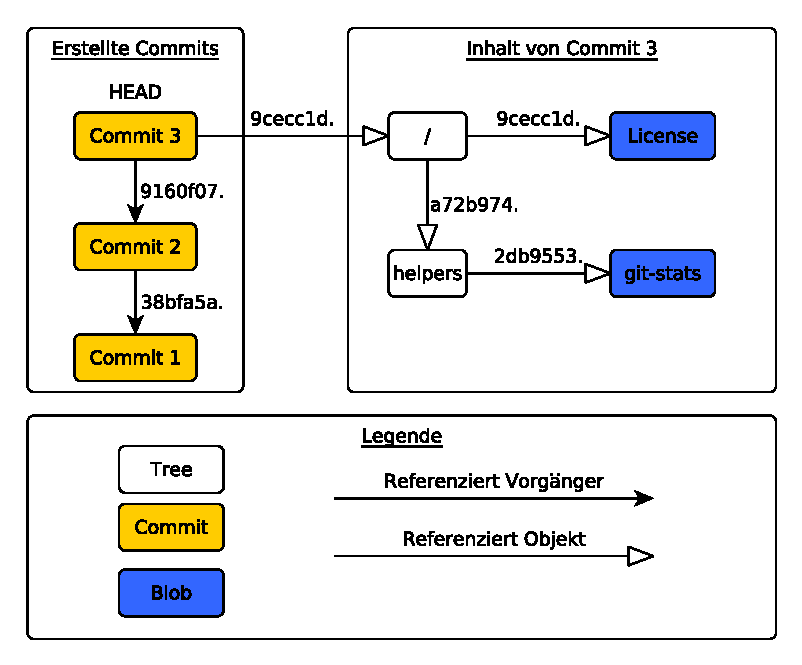
\includegraphics[scale=0.75]{images/objectmodel.eps}
  \caption{Objektmodell zum Beispiel aus Abschnitt \ref{sec:first_commits}.
  Angelehnt an \cite[S.~53]{gitosp}}.
  \label{fig:objectmodel}
\end{figure}

\subsubsection{Commit}\label{sec:commitobject}
Ein Commit-Objekt enthält neben den Daten aus Listing
\ref{lst:git_show_first_commit} eine Referenz zu \textbf{einem} \textit{tree}
und ggf. einem vorhergehenden Commit (engl. \textit{parent}). Im Fall eines
Merge-Commits (Abbildung \ref{fig:merge}) werden entsprechend so viele
Vorgänger referenziert, wie Branches zusammengeführt wurden. Hier wird jeweils
auf \gls{HEAD} des jeweiligen Branches referenziert. Der in einem Commit
referenzierte \textit{tree} ist immer ein Verweis auf einen sogenannten
\textit{top-level-tree} (\texttt{/}). Dieser referenziert die Wurzel des
entstandenen Objektbaums und enhält keinen Dateinamen (Abbildung
\ref{fig:objectmodel}).

Dadurch, dass jeder Commit seinen vorhergehenden Commit referenziert, entsteht ein
gerichteter azyklischer Graph, bei dem ein Knoten durch einen Commit und Kanten
durch Referenzen repräsentiert werden. Ein weiterer Vorteil dieser
Vorgehensweise ist, dass in dem Commit nicht immer alle enthaltenen Objekte neu
gespeichert werden, sondern nur diejenigen, die verändert wurden. Alle anderen
referenzieren das ursprünglich angelegte \textit{blob} Objekt. Dieser Effekt
wird als Deduplizierung bezeichnet und führt dazu, dass ein Repository, in dem
eine Datei viele Male existiert, bzw. referenziert wird, kaum größer ist als ein
Repository mit nur dieser einen Datei. \cite[56-57]{gitosp}

\eqlst{listings/git_show_raw.lst}{lst:git_show_raw}{Ausgabe eines Commits im
\textit{raw} Format}

Zusätzlich unterscheidet Git noch den Committer vom Autor. Diese können sich
unterscheiden, wenn Commits z.B. einen Reviewprozess durchlaufen müssen und
nicht von dem Autor selbst in das aktuelle Repository integiert werden (Listing
\ref{lst:git_show_raw}).

\subsubsection{Tag}\label{sec:tagobject}
Ein \gls{tag} markiert einzelne Commits. Hierzu werden Versionsnummern als
Namen verwendet (Abschnitt \ref{sec:tag}). Neben der \textit{SHA-1-ID} des zu
referenzierenden Commits wird ein Tagname, der Typ und der Autor
(\textit{tagger}) mit Name und Mailadresse gespeichert. Je nach Art des Tags
kann optional noch eine Beschreibung angegeben werden. Bei Tags ist nicht nur
die Prüfsumme, sondern auch der Name eindeutig. Wird versucht, ein Tag mit einem
bereits existierenden Namen zu erzeugen, reagiert Git mit einer
Fehlermeldung und lehnt das Erstellen entsprechend ab.

Git unterscheidet zwischen drei Arten von Tags:

\begin{enumerate}
\item \textbf{Lightweight Tags:} Dieser Typ ist die einfachste Variante. Er
enthält neben den benötigten Daten wie Autor, Commitreferenz und Prüfsumme
lediglich den Namen. Erzeugt wird er mit dem Befehl:

\eqlst{listings/git_light_tags.lst}{lst:git_light_tags}{Einen leichtgewichtigen
Tag anlegen}

\item \textbf{Annotated Tags:} Annotated bedeutet nichts anderes als
kommentiert. Zusätzlich zu den Daten aus den \textit{Lightweight Tags} wird
hier wie bei einem Commit ein Texteditor geöffnet. Alternativ kann auf der
Kommandozeile ebenfalls mit dem Parameter \texttt{-m} eine Beschreibung
übergeben werden.

\eqlst{listings/git_annotated_tags.lst}{lst:git_annotated_tags}{Einen
kommentierten Tag anlegen}

\item \textbf{Signierte Tags:} Voraussetzung für diese Art von Tags ist ein
vorhandener privater \textit{GPG-Key}. Diese Tags werden mit einer Signatur
versehen, die von anderen entsprechend überprüft werden kann, um die Identität
des Autors eindeutig zu verifizieren\footnote{\url{https://gnupg.org}}.
Erstellt werden signierte Tags mit dem zusätzlichen Parameter \texttt{-s}:

\eqlst{listings/git_signatured_tags.lst}{lst:git_signatured_tags}{Signierte
Tags anlegen}

Zuvor muss Git der zu verwendende Schlüssel noch bekannt gemacht werden. Das
kann mit folgendem Befehl erreicht werden:

\eqlst{listings/git_add_key.lst}{lst:git_add_key}{GPG-Key hinzufügen}
\end{enumerate}

\subsubsection{Branch}\label{sec:branchobject}
Eine einfache Antwort auf die Frage, warum ein Branch kein Objekt ist, liefert
die Ausgabe der Referenzdatei des Branches \textit{master}:

\eqlst{listings/cat_master.lst}{lst:cat_master.lst}{Den Inhalt der Referenz
\textit{master} ausgeben}

Die ausgegebene Prüfsumme ist in diesem Fall lediglich die \textit{SHA-1-ID}
des letzten Commits aus Abschnitt \ref{sec:first_commits}. Branches sind
einfache Textdateien, die eine \textit{Commit-ID} zu einem referenzierten
Commit enthalten. Da diese Referenz veränderbar ist und keine weiteren
Informationen enthält, wird hier kein weiterer Objekttyp benötigt. Da der Name
des Branches direkt von der erstellten Referenzdatei abhängig ist, sind auch
die Namen eindeutig.

Neben der fortgeschrittenen Manipulation von Git Objekten, gehen die Autoren
Scott Chacon und Ben Straub in \cite[S.~408-418]{progit} ausführlicher
auf die Objektverwaltung ein.

\subsection{Bäume}\label{sec:trees}
Git organisiert das Repository in drei verschiedenen Bereichen. Scott Chacon,
einer der Autoren von \cite{progit}, spricht in einem seiner
Vorträge \cite{link:talesoftrees} von drei Bäumen \textit{HEAD}, \textit{Index}
und dem \textit{Work Tree}.

Der \textit{Work Tree} (Abschnitt \ref{sec:workingtree}) wurde bereits als
Arbeitsbereich angesprochen. Mit \textit{\gls{HEAD}} ist neben dem Verweis auf
den neuesten Commit auch im weitesten Sinne das Repository gemeint. Das
\gls{repository} dient als Datenspeicher für alle Commits, deren Inhalte und
Historie. Der Index (Abschnitt \ref{sec:index}) in Git stellt im Vergleich zu
vorherigen Versionskontrollsystemen eine Neuerung dar. Der Index ist ein
Bereich zwischen dem \gls{repository} und dem Arbeitsbereich. Er dient dazu,
den nächsten \textit{\gls{HEAD}} bzw. Commit vorzubereiten. Die Befehle
\texttt{\$ git add}, \texttt{\$ git reset} und \texttt{\$ git commit} arbeiten
auf diesen drei Bereichen. \cite[34-35]{gitosp}

\begin{figure}[h]
    \centering
    \includegraphics[scale=0.60]{images/trees.eps}
    \caption{\textit{Work Tree}, \textit{HEAD} und Index. Angelehnt an
    \cite[34]{gitosp}}.
    \label{fig:trees}
\end{figure}

\subsection{Ergänzende Befehle}\label{sec:commands}
Die bisher verwendeten Befehle werden in diesem Abschnit um weitere ergänzt,
die für die alltägliche Arbeit mit Git sinnvoll sind\footnote{Weitere siehe
hierzu \cite{gitosp}, \cite{progit} oder \cite{gitwf}.}.

Alle Git Befehle bieten eine Vielzahl an Optionen. So verstehen viele der
Befehle, die Änderungen an dem Repository vornehmen, den Parameter
\texttt{\-{}\-{}dry-run}, der es ermöglicht, Vorgänge erst zu simulieren.
Außerdem bieten die meisten Git Befehle mit \texttt{-v} eine umfangreichere
Ausgabe (engl. \textit{verbose}) an. Eine Übersicht über die unterstützten
Optionen kann mit den unter Linux üblichen Methoden angezeigt werden. So z.B.
mit \texttt{\$ git help <Befehl>} oder mit dem klassischen Aufruf der Manpage
\texttt{\$ man git <Befehl>}.

Viele der Befehle erwarten ein bestimmtes Objekt als Argument. So finden sich
häufig Argumente, die als \textit{tree-ish} oder \textit{commit-ish} bezeichnet
werden. Damit sind aber lediglich entsprechende Objekte gemeint, die z.B. einen
Tree referenzieren. So benötigt \texttt{\$ git ls-tree} aus Abschnitt
\ref{sec:objectmodel} ein \textit{tree-ish} und \texttt{\$ git show} kann auf
allen Objekten aus Abschnitt \ref{sec:objectmodel} arbeiten. \cite[52]{gitosp}

\subsubsection{Dateien hinzufügen}\label{sec:gitadd}
Mit \texttt{\$ git add} können grundsätzlich Dateien hinzugefügt werden. Der
Befehl selbst bietet, wie fast alle Git Befehle, eine Vielzahl an Optionen.
Eine sei an dieser Stelle besonders erwähnt, \texttt{\$ git add -p}. Das
\texttt{-p} ermöglicht, die durchgeführten Änderungen an den Dateien selektiv
auf den Index zu legen und somit für einen Commit vorzumerken. Das kann
hilfreich sein, um Änderungen an verschiedenen Teilen in einzelne
\glspl{commit} aufzuteilen oder bestimmte Änderungen
wegzulassen. \cite[S.~36-37]{gitosp}

\subsubsection{Dateien verschieben} Will man Dateien verschieben, kann man den
Befehl \texttt{\$ git mv} benutzen. Dieser Befehl arbeitet ähnlich wie der
gleichnamige Linux-Befehl. Um den Vorgang zu erzwingen, wenn beispielsweise
die Zieldatei schon existiert, kann der Parameter \texttt{-f} für
\textit{force} angegeben werden. Die Dateien können aber auch genauso mit unter
Linux üblichen Mitteln wie \texttt{cp, rm, mv} etc. verschoben werden.
Anschließend muss die Änderung lediglich mit dem Befehl \texttt{\$ git add}
hinzugefügt werden.\cite[S.~43-44]{gitosp}

\eqlst{listings/git_mv.lst}{lst:git_mv}{Dateien verschieben}

\subsubsection{Dateien entfernen}
Der Befehl \texttt{\$ git rm} steht für \textit{remove}, bewirkt aber nicht das
Gegenteil von \texttt{add}. Dieser Befehl entfernt, vergleichbar mit dem
Linux-Befehl, Dateien oder Verzeichnisse. Um nicht leere Verzeichnisse zu
löschen, muss noch ein \texttt{-r} für rekursiv angegeben werden. Wenn Dateien
bereits verändert wurden, kann zusätzlich noch mit einem \texttt{-f} der
Vorgang erzwungen werden.

\eqlst{listings/git_rm.lst}{lst:git_rm}{Dateien entfernen}

Das Entfernen von Dateien aus dem Repository kann aber genauso mit unter Linux
üblichen Mitteln vorgenommen werden. Die Änderungen müssen dann mit \texttt{\$
git add} dem Index hinzugefügt werden. Die Dateien werden aber nicht
vollständig entfernt. Der neu erstellte Commit verweist lediglich nicht mehr
auf das entsprechende Objekt (Abschnitt \ref{sec:commitobject}).
\cite[S.~43-44]{gitosp}

\subsubsection{Tags verwalten}\label{sec:managetags}
Die eindeutige Identifikation von Versionen bzw. konkreten Zuständen eines
Repositories mit \gls{sha1} Prüfsummen ist aus technischer Sicht problemlos.
Als Mensch hingegen kann man sich solche Prüfsummen weder gut merken, noch geht
aus den Prüfsummen eine Historie hervor. Git ermöglicht es mit dem Befehl
\texttt{\$ git tag} Objekte, zumeist Commits, namentlich zu markieren. Als
Namen dieser Markierungen wird man in der Praxis eine Vielzahl an Varianten
finden. Eine durchaus übliche ist aber die Kombination aus drei bis vier
fortlaufenden Zahlen. Um den Tag zusätzlich zu identifizieren, kann hier auch
noch ein Präfix, z.B. \texttt{release/} oder \texttt{v} verwendet werden. Wie
Tags angelegt und angezeigt werden, ist in Listing \ref{lst:git_first_tag} und
Listing \ref{lst:git_list_first_tag} gezeigt.  Ebenso wurde in Abschnitt
\ref{sec:tagobject} bereits auf die verschiedenen Typen von Tags eingegangen.
Ergänzend hierzu sei noch erwähnt, dass Tags mit dem zusätzlichen Parameter
\texttt{-d} gelöscht und mit \texttt{-f} überschrieben werden können. Das
Herunterladen von Tags erfolgt über \texttt{\$ git fetch} (Abschnitt
\ref{sec:distributed}) und das Veröffentlichen über \texttt{\$ git push}:

\eqlst{listings/git_push_tag.lst}{lst:git_push_tag}{Einen Tag veröffentlichen}

Um alle lokalen Tags zu veröffentlichen, kann der \texttt{\$ git push} Befehl auch mit
dem Parameter \texttt{--tags} kombiniert werden. \cite[70-71,162-163]{gitosp}

\eqlst{listings/git_push_all_tags.lst}{lst:git_push_all_tags}{Alle erzeugten
Tags veröffentlichen}

\subsubsection{Branches verwalten}
Ähnlich wie bei Tags markiert auch ein Branch eine \gls{sha1} Prüfsumme, in
diesem Fall die eines Commits. Im Gegensatz zu Tags sind diese lediglich
dynamische Referenzen. Da hier nur eine Textdatei mit der Referenz erstellt
werden muss, ist der Vorgang entsprechend schnell. Das Erstellen eines
Branches benötigt als Argument mindestens einen eindeutigen Namen (Abschnitt
\ref{sec:branchobject}). Wenn keine Referenz auf einen Commit übergeben wird,
wählt Git einfach den aktuellen \textit{\gls{HEAD}}. Das folgende Beispiel
erstellt einen Branch namens \textit{topic} von der Referenz \textit{master}.

\eqlst{listings/git_branch.lst}{lst:git_branch}{Einen Branch anlegen}

Um auf einen anderen Branch zu wechseln, kann der Befehl \texttt{\$ git checkout
<name>} benutzt werden.

In bestimmten Situationen verweigert Git den Checkout, beispielsweise wenn eine
Datei überschrieben würde oder ein Wechsel des Branches zusätzliche Änderungen
an einer lokal geänderten Datei zur Folge hätte. Der Parameter \texttt{-f}
erzwingt auch hier den gewünschten Vorgang. Mit \texttt{\$ git checkout} können
auch Branches angelegt und direkt darauf gewechselt werden:

\eqlst{listings/git_checkout.lst}{lst:git_checkout}{Einen Branch anlegen und
darauf wechseln}

Der Befehl \texttt{\$ git branch} unterstützt noch weitere Parameter. So kann
mit den Parametern \texttt{-d/-D}\footnote{Der Parameter \texttt{-D} wird
benötigt, wenn auf dem Branch Objekte sind, die noch nicht dem aktuellen Branch
hinzugefügt wurden \cite[67]{gitosp}.} ein Branch gelöscht werden oder mit
\texttt{-m} ein Branch umbenannt werden. Lokale Branches können mit
\texttt{-l}\footnote{Das ist das Standardverhalten, wenn kein Parameter
übergeben wird.} angezeigt werden, entfernte aus dem entfernten Repository mit
\texttt{-r} und alle zusammen mit \texttt{-a}. \cite[65-67]{gitosp}

Weitere Details zur Arbeit mit Branches sind beispielsweise in \cite[388-389,
408-415]{cd} und \cite[56-88]{progit} enthalten.

\subsubsection{Historie untersuchen}\label{sec:arch}
In Abschnitt \ref{sec:first_commits} wurde bereits auf \texttt{\$ git
whatchanged} eingegangen. Wie bereits erwähnt, verbirgt sich dahinter der
Befehl \texttt{\$ git log}. Mit diesem Befehl kann die Versionshistorie des
\glspl{repository} untersucht werden. Dies wird hier am Beispiel aus dem
genannten Abschnitt gezeigt:

\eqlst{listings/git_log.lst}{lst:git_log}{Versionsgeschichte mit \texttt{log}
anzeigen}

Der Unterschied zu Listing \ref{lst:first_git_whatchanged} ist die etwas
reduzierte Ausgabe. Um die Ausgabe noch weiter einzuschränken, kann der
Parameter \texttt{--oneline} genutzt werden.

\eqlst{listings/git_log_oneline.lst}{lst:git_log_oneline}{Versionsgeschichte
einzeilig anzeigen}

Auch kann die Ausgabe auf einen oder mehrere Commits eingeschränkt werden.
Hierzu muss zusäzlich die entsprechende \textit{SHA-1-ID} oder die
Referenz übergeben werden. Soll ein bestimmter Bereich untersucht werden, kann
der Anfang mit \texttt{..} vom Ende getrennt werden:

\eqlst{listings/git_log_range.lst}{lst:git_log_range}{Versionsgeschichte auf
einen Bereich einschränken}

Die Trennung mit zwei Punkten wird auch von vielen anderen Befehlen verstanden,
so wie beispielsweise von \texttt{\$ git diff} oder \texttt{\$ git show} (Abschnitt
\ref{sec:first_commits}). Die Auswahl des angezeigten Bereichs erfolgt immer
exklusive des ersten und inklusive des zweiten (nach \texttt{..}) angegebenen
Commits. \cite[45-48]{gitosp}

\subsubsection{Aktuelle Änderungen anzeigen}\label{sec:gitdiff}
Veränderte Dateien können entweder im Arbeitsbereich (Abbildung
\ref{fig:trees}) oder bereits auf dem Index vorliegen (Abschnitt
\ref{sec:gitadd}). Für die Anzeige, wird \texttt{\$ git diff} verwendet.
Wird der letzte Absatz aus der Lizenzdatei (Abschnitt \ref{sec:first_commits})
entfernt, zeigt \texttt{\$ git status} folgende Situation:

\eqlst{listings/git_status_wk.lst}{lst:git_status_wk}{Status des
Arbeitsbereichs anzeigen}

Der Befehl \texttt{\$ git diff} führt nun zu folgender Ausgabe im \textit{Unified-Diff}
Format:

\eqlst{listings/git_diff_wk.lst}{lst:git_diff_wk}{Änderungen auf Arbeitsbereich anzeigen}

Ein anschließendes \texttt{\$ git add LICENSE}, führt zum Verschieben auf den
Index und \texttt{\$ git diff} zu einer leeren Ausgabe:

\eqlst{listings/git_status_staged.lst}{lst:git_status_staged}{Status des Index anzeigen}

Um die Änderungen auf dem Index zu betrachten, muss der Befehl \texttt{\$ git
diff} um den Parameter \texttt{--staged} ergänzt werden\footnote{Die Parameter
\texttt{--staged} und \texttt{--cached} können synonym verwendet
werden und stehen in diesem Fall für das Betrachten der \textit{Staging
Area} (Abschnitt \ref{sec:index}).}. \cite[26-29]{progit}
